\documentclass[a4paper, 14pt]{extarticle}

\usepackage{ifluatex}
\usepackage{ifpdf}

\ifluatex
\usepackage{fontspec}
\defaultfontfeatures{Renderer=Basic,Ligatures={TeX}}
\setmainfont{CMU Serif}
\setsansfont{CMU Sans Serif}
\usepackage{polyglossia}
\setdefaultlanguage{russian}
\setotherlanguage{english}
\setmainfont{CMU Serif}
\newfontfamily{\cyrillicfont}{CMU Serif}
\setsansfont{CMU Sans Serif}
\newfontfamily{\cyrillicfontsf}{CMU Sans Serif}
\setmonofont{CMU Typewriter Text}
\newfontfamily{\cyrillicfonttt}{CMU Typewriter Text}
\else
\ifpdf 
\usepackage[T2A]{fontenc}
\usepackage[utf8]{inputenc}
\usepackage[english,russian]{babel}
\typeout{PDF only}
\fi
\fi

\usepackage[left=1cm,right=1cm,top=2cm,bottom=2cm]{geometry}
%%% Дополнительная работа с математикой
\usepackage{amsfonts,amssymb,amsthm,mathtools} % AMS
\usepackage{amsmath}
\usepackage{icomma} % «Умная» запятая: $0,2$ — число, $0, 2$ — перечисление

\usepackage{mathrsfs} % Красивый матшрифт

%% Перенос знаков в формулах (по Львовскому)
\newcommand*{\hm}[1]{#1\nobreak\discretionary{}
  {\hbox{$\mathsurround=0pt #1$}}{}}

%%% Работа с картинками

\usepackage{graphicx}  % Для вставки рисунков
\graphicspath{ {images/} }
\setlength\fboxsep{3pt} % Отступ рамки \fbox{} от рисунка
\setlength\fboxrule{1pt} % Толщина линий рамки \fbox{}
\usepackage{wrapfig} % Обтекание рисунков и таблиц текстом

\usepackage[dvipsnames]{xcolor}
\usepackage{verbatim}
\usepackage{hyperref}

\usepackage{listings}

\lstdefinelanguage{JavaScript}{
  keywords={let, typeof, new, true, false, catch, function, return, null, catch, switch, var, if, in, while, do, else, case, break, const},
  keywordstyle=\color{blue}\bfseries,
  ndkeywords={class, export, boolean, throw, implements, import, this,},
  ndkeywordstyle=\color{darkgray}\bfseries,
  identifierstyle=\color{black},
  sensitive=false,
  comment=[l]{//},
  morecomment=[s]{/*}{*/},
  commentstyle=\color{green}\ttfamily,
  stringstyle=\color{red}\ttfamily,
  morestring=[b]',
  morestring=[b]",
  escapechar=|
}

\lstset{
  language=JavaScript,
  extendedchars=true,
  basicstyle=\small\ttfamily,
  showstringspaces=false,
  breakatwhitespace=true,
  showspaces=false,
  numbers=left,
  numberstyle=\footnotesize,
  numbersep=9pt,
  tabsize=2,
  keepspaces=true,
  breaklines=true,
  showtabs=false,
  captionpos=b
  escapechar=|,
  frame=single ,
  commentstyle=\itshape ,
  frameshape={RYR}{Y}{Y}{RYR},
  stringstyle =\bfseries,
}

\usepackage{autobreak}

\newcommand*{\function}[2]{\texttt{\textcolor{Red}{function} \textcolor{Purple}{#1}(#2)}\linebreak}

\newcommand*{\prototype}[3][]{\texttt{\textcolor{Orange}{#2}.\textcolor{Blue}{prototype}.\textcolor{Purple}{#3} = \textcolor{Red}{function}(#1)}\linebreak}

\usepackage{titlesec}

\setcounter{secnumdepth}{4}

\titleformat{\paragraph}
{\normalfont\normalsize\bfseries}{\theparagraph}{1em}{}
\titlespacing*{\paragraph}
{0pt}{3.25ex plus 1ex minus .2ex}{1.5ex plus .2ex}

\usepackage{multicol}
\setlength{\columnsep}{1cm}

\usepackage[most]{tcolorbox}

\newtcolorbox{leftBox}{
  colback=white,colframe=black, 
  width = 0.97\linewidth,
  sharp corners = southwest,
}

\usepackage{newfloat,caption,float}
\usepackage{capt-of}

\DeclareFloatingEnvironment[
  fileext = loe,
  listname = Задача,
  name = Задача.,
  placement = H,
  within = none,
  ]{application}
\captionsetup[application]{labelfont=md}

\DeclareFloatingEnvironment[
  fileext = loe,
  listname = Рис,
  name = Рис.,
  placement = H,
  within = none,
  ]{image}
\captionsetup[image]{labelfont=md}

\usepackage{tikz,tikz-3dplot}

\renewcommand{\lstlistingname}{Листинг}% Listing -> Листинг


\newcommand*{\task}[4]{
  \begin{minipage}[t]{\linewidth}
  \begin{multicols}{2}
    #1\\\\
    Ответ: $#2$\\
    \includegraphics[width=0.4\textwidth]{#3}
  \end{multicols}
  \captionof{application}{Пример генерации задания с помощью #4}
\end{minipage}
}

\usepackage{setspace}

\begin{document}


\begin{center}
	\hfill \break
	\large{МИНОБРНАУКИ РОССИИ}\\
	\footnotesize{ФЕДЕРАЛЬНОЕ ГОСУДАРСТВЕННОЕ БЮДЖЕТНОЕ ОБРАЗОВАТЕЛЬНОЕ УЧЕРЕЖДЕНИЕ}\\
	\footnotesize{ВЫСШЕГО ПРОФЕССИОНАЛЬНОГО ОБРАЗОВАНИЯ}\\
	\small{\textbf{«ВОРОНЕЖСКИЙ ГОСУДАРСТВЕННЫЙ УНИВЕРСИТЕТ»}}\\
	\hfill \break
	\normalsize{Факультет компьютерных наук}\\
	\hfill \break
	\normalsize{Кафедра цифровых технологий}\\
	\hfill\break
	\hfill \break
	\hfill \break
	\hfill \break
	\large{Программная реализация (на языке JavaScript) алгоритмов генерации ФОС ЕГЭ по геометрии в 2025 году}\\
	\hfill \break
	\hfill \break
	\hfill \break
	\hfill \break
	\hfill \break
	\normalsize{Курсовая работа\\
		\hfill \break
		Направление  020301 Математика и компьютерные науки\\

		\hfill \break
	}\\
	\hfill \break
	\hfill \break
\end{center}
\hfill \break

\normalsize{
	\begin{tabular}{cccc}
		Зав.кафедрой & \underline{\hspace{3cm}} & док.физ.-мат.н.,  проф. & С.Д. Кургалин    \\\\
		Обучающийся  & \underline{\hspace{3cm}} &                       & Е.Ю. Колесникова \\\\
		Руководитель & \underline{\hspace{3cm}} & доц.кан.физ-мат.н,  проф. & Н.П Стадная    \\\\
	\end{tabular}
}\\
\hfill \break
\hfill \break
\begin{center} Воронеж 2025 \end{center}
\thispagestyle{empty} % выключаем отображение номера для этой страницы

% КОНЕЦ ТИТУЛЬНОГО ЛИСТА

\setstretch{1.5}

\tableofcontents


\section*{Введение}
\addcontentsline{toc}{section}{Введение}
Единый государственный экзамен (ЕГЭ)~— централизованно проводимый в Российской
Федерации экзамен в средних учебных заведениях — школах, лицеях и гимназиях,
форма проведения ГИА (Государственной Итоговой Аттестации) по образовательным программам среднего общего образования.
Служит одновременно выпускным экзаменом из школы и вступительным экзаменом в вузы.

Но за время обучения в 9, 10 и 11 классе при подготовке к ОГЭ и ЕГЭ школьники сталкиваются с дефицитом заданий по определённым категориям.
Так, за последние 5 лет в список заданий ЕГЭ были добавлены новые задания под номером 1 по теме «Округление с недостатком» и «Округление с избытком», так же задания под номером 15 «Проценты и округление»,21 задания « Текстовые задачи», количество которых для прорешивания было мало. 
Ко всему прочему в задании номер 7 по теме «Числовые неравенства, координатная прямая -числа на прямой» банк заданий расходуется при подготовке с невероятной скоростью:
так как это преимущественно графические задания, решение их занимает менее минуты, а их составление вручную занимает несоразмерно много времени. ОГЭ и ЕГЭ является относительно неизменяемым экзаменом, поэтому все материалы, которые уже были выложены в открытый доступ, имеют полные решения, что приводит к списыванию учениками.

При этом существуют задания со вспомогательным чертежом. Чаще всего для целого ряда заданий используется одна и та же иллюстрация, которая не всегда соответствуют условиям задачи, а иногда отвлекает от решения.
Проект «Час ЕГЭ» позволяет решить все эти проблемы.

(«Час ЕГЭ»)~\cite{chas-ege} — компьютерный образовательный OpenSource-проект, предназначенный для помощи учащимся
старших классов при подготовке к тестовой части единого государственного экзамена.

Задания в «Час ЕГЭ» генерируются случайным образом по специализированным алгоритмам,
называемых шаблонами, каждый из которых
охватывает множество вариантов соответствующей ему задачи. Для
пользователей
предназначены четыре оболочки (режима работы): «Случайное задание», «Тесты на печать»,
«Полный тест» и «Мини-интеграция».
«Час ЕГЭ» является полностью открытым (код находится под лицензией GNU GPL 3.0)
и бесплатным.
В настоящее время в проекте полностью реализованы тесты по ЕГЭ по математике профильного уровня с кратким
ответом (бывшая «часть В»).~\cite{fipi}
Планируется с течением времени включить в проект тесты по другим предметам школьной
программы.

Первую главу посвятим обзору шаблонов для номеров (21, 15, 1 из ЕГЭ базовой)~\cite{egemath}.
Во второй главе рассмотрим функцию добавленному для упрощения отрисовки прямых для (7 задания ОГЭ)~\cite{ogemath}.



\section{Генерация текстовых задач}

В Первом разделе представлены работы, связанные Текстовыми задачами. 
%Работа велась на языке \texttt{JavaScript}, с использованием вспомогательных функций для визуализации и генерации условий.
Так как в 
%15, 21 "текстовые задачи"
%рассказать про декорации, про chislitlx(пулл реквест с r2), сочетания 
%предварительные сведения (функции, кратко ,генассерт и тп)
%платформа час-ЕГЭ (то что сделала сама "хвалюсь") для "реализации задачи мною были разработаны" и тп, 
% то что существует - описываю как факт (а.к.а предварительные сведения)
% 4 1)отдельно (формулы) естественно появляется обратная задача. 2)Сослаться на Латех (MathJax) основные команды которыми пользуемся в Латехе texfrag и тп 
%7 делится на две главы. Задача с чертежом коорд.оси (предвор сведения, разработанные библ функции, шаблоны)
% вторая - задача на сравнение чисел (как устроено округление,autoLateX )
% в заключении написать количество вып задач по категориям 
%в данной главе (тото это тамто и тп)
% не менее 10 шаблонов сумарно затронув каждую категорию 
% где-то 45-50 страниц....
% про расвнение чисел очень долго целых чисел не было, все числа были дробные, 0.1+0.2!=0.3 надо быть осторожным и тп расскажи!! 
%захожу в калатог, через меню переключаемся на тест на печать внимательно (?) выставить нулями все задания кроме того что нужно ставить галочку " экспорт в латех" 
%ставим запуск,жду,думаю, падает зипка с задачами в латехе, в перемешку 
%исходная задача/код/полученная задача (сгенерин текст)
При построении текстовых шаблонов задач важно обеспечить как вариативность формулировок, так и корректность числовых и языковых выражений. Для этого в проекте применяются следующие инструменты.

\subsection{Декорации}

Чтобы увеличить количество уникальных вариантов задач, сохраняя их математическую суть, используются так называемые ``декорации''~--- элементы окружения, которые можно менять без потери смысла задачи: имена персонажей, место действия, цель, контекст. 
Для этого создаются массивы строк, а функция \texttt{iz()} случайным образом выбирает элемент из массива.

Пример:
\begin{lstlisting}
let contract = ['о дружбе', 'во избежание двойного налогообложения',
    'о безвизовом режиме', 'об экологической среде',
    'по гуманитарным вопросам', 'по вопросам безопасности'].iz();
\end{lstlisting}
\textsl{Задача №514913.}
\lstinputlisting[]{code/21/514913.js} 

Если необходимо выбрать два случайных, но не повторяющихся элемента, используется форма \texttt{iz(2)}:  
\begin{lstlisting}
let tapeName = sklonlxkand(['лента', 'верёвка', 'нитка'].iz(2));
\end{lstlisting}
\textsl{Задача №2434.}
%добавить пример до/после 
\lstinputlisting[]{code/21/2434.js} 
До:
После:
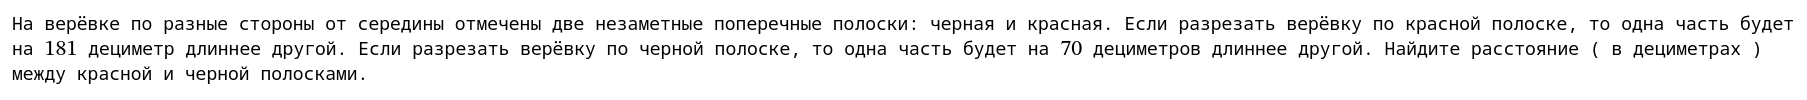
\includegraphics[width=1.4\textwidth]{2434-21-1.png}
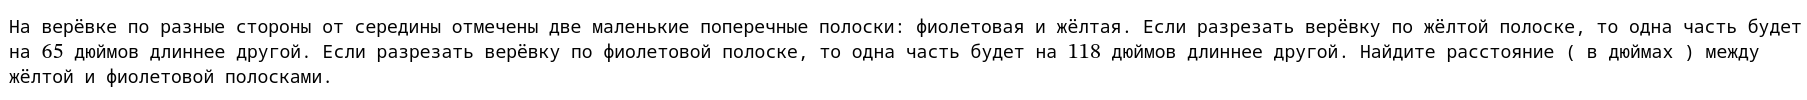
\includegraphics[width=1.4\textwidth]{2434-21-2.png}

Чтобы каждый раз не задавать список декораций,у нас есть несколько заготовленных, которые используются от задаче к задаче. Например \texttt{om.meltov={}} и они могут быть рассписаны даже по нескольким падежам.

Например: 
\begin{lstlisting}
om.meltov={}
om.meltov.ie = ['фонарик', 'флакон шампуня', 'флэшка', 'компакт-диск', 'сувенир', 'матрёшка', 'магнит на холодильник', 'сборник тестов для подготовки к ЕГЭ', 'тетрадь', 'учебник', 'цветочный горшок'];
\end{lstlisting}
В задаче же благодаря этому можно записать короче:
\begin{lstlisting}
let item = sklonlxkand((om.meltov.ie).iz());
\end{lstlisting}
\textsl{Задача №314120.}

Как вы могли заметить, некоторые декорации являются словосочетанием, например "флакон шампуня", "цветочный горшок", "магнит на холодильник" и так далее. И для более коректной работы \texttt{.ie} и других падежей у нас есть словарь \texttt{lxsoch.js}
Однако недавно было выявленно, что если рядом со словосочетанием стоит число, то оно должно изменяться. например "3 цветочных горшка" или " 4 флакона шампуня". Они очень схожи с родительным падежом множественного числа, но отличаются. Так что мною был добавлен в  
\texttt{lxsoch.js} \texttt{.r2}. Это падеж, в котором учтено изменения слова из-за числительного. 
%добавить пример Саши?

\subsection{Склонения сушествительных}

В силу особенностей русского языка слова должны корректно изменяться по падежам и числам. Для этого применяется функция \texttt{sklonlxkand}, позволяющая генерировать правильные словоформы.  
После выбора слова к нему можно обратиться по падежу и числу. Например, \texttt{.ie} означает именительный падеж, единственное число.  

Пример использования:
\begin{lstlisting}
let typeOfFlowerInVases =
  sklonlxkand(['роза','гвоздника','ромашка','лилия',
               'мак','ирис','лаванда','мимоза'].iz());
NAtask.setTask({
  text: 'На прилавке цветочного магазина стоят три вазы с '
    + typeOfFlowerInVases.tm + ': ' + vaseColor[0] + 'ая, '
    + vaseColor[1] + 'ая, ' + vaseColor[2] + 'ая.' 
    + ' Слева от ' + vaseColor[2] + 'ой вазы '
    + chislitlx(leftOfThirdVase, typeOfFlowerInVases, '$')
    + ', справа от ' + vaseColor[0] + 'ой вазы '
    + chislitlx(righttOfFirstVase, typeOfFlowerInVases, '$') + '. '
    + 'Всего в вазах '
    + chislitlx(allFlowerInVases, typeOfFlowerInVases, '$') + '. '
    + 'Сколько ' + typeOfFlowerInVases.rm + ' в '
    + vaseColor[1] + 'ой вазе?',
  answers: secondVaseCountFlower,
});
\end{lstlisting}
\textsl{Задача №515842.}

\lstinputlisting[]{code/21/515842.js} 
До:
После:
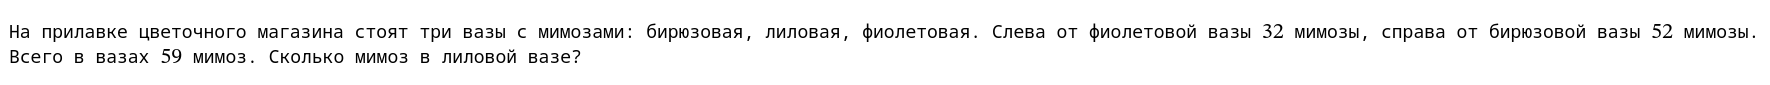
\includegraphics[width=1\textwidth]{515842-21.png}    

Для корректного согласования числительных с существительными используется функция \texttt{chislitlx}. Она автоматически выбирает нужную форму слова в зависимости от числа.  
% написать про ceil() 
%добавить примеры до/после
Пример:
\begin{lstlisting}
let numberOfApartamentPerFloor = sluchch(3, 12, 1);
NAtask.setTask({
  text: 'В доме, в котором живет ' + nameOfPerson + ', ' +
    '$' + floorNumber + '$ этажей и несколько подъездов. На каждом этаже находится по ' +
    chislitlx(numberOfApartamentPerFloor, 'квартира', '$') + '. '
    + nameOfPerson + ' живет в квартире №' + '$' + apartamentNumber + '$' + '. '
    + 'В каком подъезде живет ' + nameOfPerson + '? ',
  answers: '$' + (apartamentNumber /
             (floorNumber * numberOfApartamentPerFloor)).ceil() + '$',
});
\end{lstlisting}
\textsl{Задача №77351.}

\subsection{Проверка условий (генерация утверждений)}

Помни во всех шаблонах вы так или иначе увидете окружение \texttt{retryWhileError}, которое ограничевает количество перезапусков, плюсом ещё и фиксирует какие проверки не были пройдены и выводить их на экран. Само собой ошибки видны только разработчикам Во время отладки.
\function{retryWhileError}{theFunction, maxIterations,maxCollectedErrors}

Пример: 
\lstinputlisting[]{code/15/509768.js}
До: 
После: 

\includegraphics[width=1\textwidth]{509768-15-1.png}  

\includegraphics[width=1\textwidth]{509768-15-2.png}  

Для контроля корректности задачи применяются функции \texttt{genAssert} и её вариации. Принцип работы:  
\begin{itemize}
    \item если условие не выполнено~--- фиксируется ошибка;
    \item шаблон перезапускается;
    \item если достигнуто максимальное количество перезапусков, выводятся накопившиеся ошибки с указанием количества.
\end{itemize}

Пример использования:
\begin{lstlisting}
let students = sl(200, 10000, 10);
let percent = sl(10, 90, 1); 
genAssert(students.kratno(100 / percent),
          "количество учащихся не кратно 100/процент");
\end{lstlisting}
\textsl{Задача №77340.}

Также часто используется функция \function{genAssertZ1000}{number, message}, проверяющая точность чисел: если у числа более трёх знаков после запятой, шаблон перезапускается.  
\function{genAssertIrreducible}{numerator, denominator, message} - проверка на несократимость дроби.

Пример:
\begin{lstlisting}
let prise = sl(100, 2000, 10);
let percentSecondMonth = sl(10, 90, 1);
let percentThirdMonth = sl(10, 90, 1);

let middlePrise = prise * (1 + [1, -1][randFirst] * 0.01 * percentSecondMonth);
let finalePrise = middlePrise * (1 + [1, -1][randSecond] * 0.01 * percentThirdMonth);

genAssertZ1000(finalePrise / 10,
               'Число имеет более 2 знаков после запятой');
\end{lstlisting}
\textsl{Задача №77349.}

\lstinputlisting[]{code/15/77349.js}
До:
После:
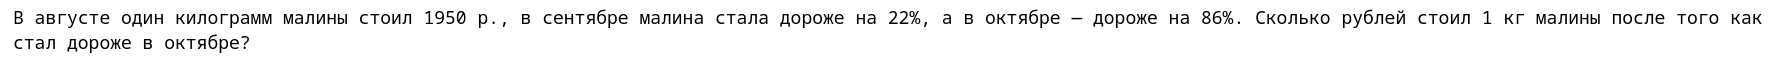
\includegraphics[width=1\textwidth]{77349-15-1.png}
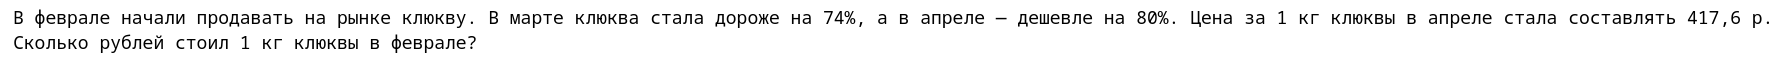
\includegraphics[width=1\textwidth]{77349-15-2.png}

В некоторых случаях может применяться \texttt{slKrome} ,он работает как \texttt{sluchch} - создает случайное число. Однако с условием что оно  отличное от
		первого параметра (первый параметр может быть числом, строкой, массивом или функцией),
		второй и третий параметры - это диапазон генерации, а четвертый параметр - шаг (по умолчанию это 1).
Пример:
\begin{lstlisting}
let mlnRuble = slKrome([100], 10, 200, 1);
\end{lstlisting}
\textsl{Задача №506346.}

\texttt{kratno} является функцией, провищяющее кратно ли данное число другому. Чаще всего используем в genAssert для проверки
Пример:
let students = sl(200, 10000, 10);
let percent = sl(10, 90, 1);
genAssert(students.kratno(100 / percent), "количество учащихся не кратко 100/процент");
\textsl{Задача №77340.}

\texttt{NAtask.modifiers.allDecimalsToStandard} мы используем в случаях работы с десятичными числами и дробями, для более коррктеного расчёта java script формул.
 Это помогает избежать излишней точности.

Пример:
\begin{lstlisting}
 let difference = sl(2, 20, 1);
        let minAngle = (360 / (2 * difference + 1));
        let maxAngle = (360 / (difference + 2));

        let result = maxAngle.floor() - minAngle.floor() - Number(maxAngle % 1 == 0 || minAngle % 1 == 0);

        NAtask.setTask({
            text: 'Три луча, выходящие из одной точки, разбивают плоскость на $3$ ' +
                'разных угла, измеряемых целым числом градусов. Наи' + moreOrLess + 'ьший угол в ' +
                chislitlx(difference, 'раз', 'v$') + ' ' + moreThanLessThan +
                ' наи' + lessOrMore + 'ьшего. Сколько значений может принимать величина среднего угла?',
            answers: result,
        });
        NAtask.modifiers.allDecimalsToStandard();
\end{lstlisting}       
\textsl{Задача №514918.}

\lstinputlisting[]{code/21/514918.js}
До:
После:

\includegraphics[width=1\textwidth]{514918-21.png}

\subsection{Разнообразие в текстовых задачах}
%не забудь вставить картинки(до и после) для каждого условия этих задачек
И самое главное для текстовых задач, возможность их разнообразить. Дело в том что изначально даётся достаочно много условий в задаче,от чего можно написать альтернативные варианты задачи. Что помогает ученикам лучше запонимать не просто последовательность решения, а принцип.
Чаще всего от изменений условия задачи на альтернативное сильно меняется и текст, по этому мы используем questions. Он позволяется разбить на несколько заданий одно и для каждого приписать свой ответ. Если же у них общее начало то можно записать его в первый text, а если одинавокое окончение то 
дописать его в postquestion.

Пример1: 
\lstinputlisting[]{code/15/506426.js} 
\textsl{Задача №506426.}
До:
После:
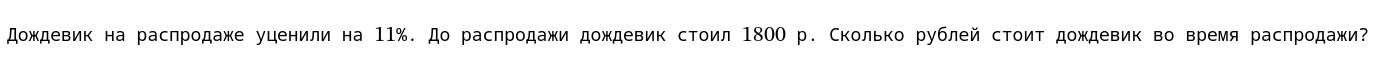
\includegraphics[width=1\textwidth]{506426-15-1.png}

\includegraphics[width=1\textwidth]{506426-15-2.png}
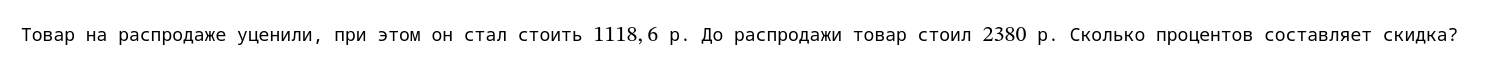
\includegraphics[width=1\textwidth]{506426-15-3.png}

Пример2:
\lstinputlisting[]{code/15/522673.js} 
\textsl{Задача №522673.}
До:
После:

\includegraphics[width=1\textwidth]{522673-15-1.png}
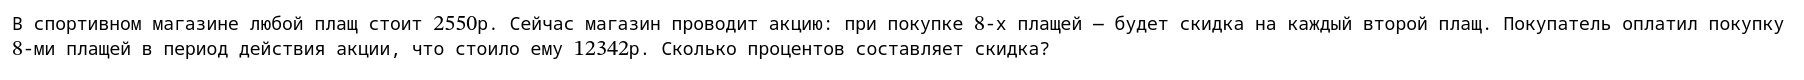
\includegraphics[width=1\textwidth]{522673-15-2.png}

\includegraphics[width=1\textwidth]{522673-15-3.png}
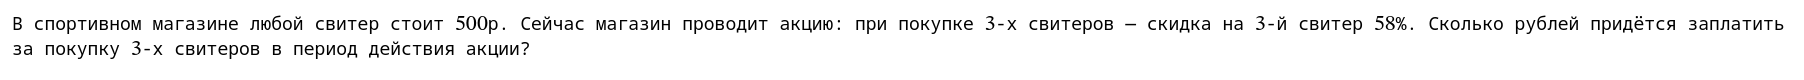
\includegraphics[width=1\textwidth]{522673-15-4.png}
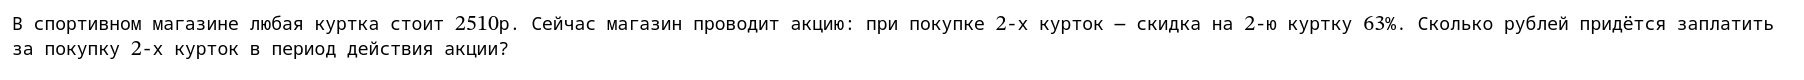
\includegraphics[width=1\textwidth]{522673-15-5.png}
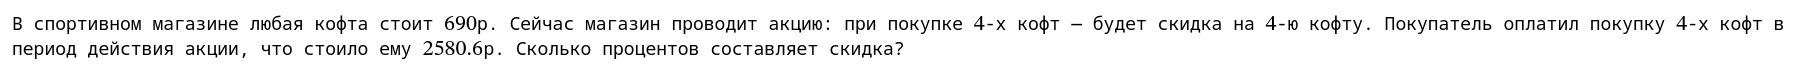
\includegraphics[width=1\textwidth]{522673-15-6.png}

\section{Задачи №4 ЕГЭ (преобразование выражений)}

% 4 1)отдельно (формулы) естественно появляется обратная задача. 2)Сослаться на Латех (MathJax) основные команды которыми пользуемся в Латехе texfrag и тп 
% тут рассказать много про MathJax
% закинуть фото ДЛЯ КАЖДОГО пункта
\subsection{Основные используемые команды}

Задачи этого вида проверяют умение подставлять значения в формулы, преобразовывать выражения (в том числе со стандартными функциями и корнями), аккуратно работать с единицами измерения и корректно представлять результат. 
В нашем генераторе текст формулировок размечается \emph{TeX}-фрагментами и рендерится через MathJax. 
При включённой опции \verb|autoLaTeX| (см. ниже) TeX-формулы можно вставлять непосредственно в строку без явного окружения \verb|$...$|.

Пример:
\begin{lstlisting}
NAtask.setTask({
			text:
				'В фирме «' + name + '» стоимость (в рублях) колодца из железобетонных колец рассчитывается по формуле $C = ' + plus + '+' + multiply + 
				' \\cdot n$, где $n$ – число колец, ' +
				'установленных при рытье колодца. ' +
				'Пользуясь этой формулой, ' +
				'рассчитайте стоимость колодца из $' + number + '$ колец.',
			answers: cost,
		});
\end{lstlisting}
\textsl{Задача №124.}

\lstinputlisting[]{code/4/124.js} 

\begin{lstlisting}
NAtask.setTask({

			text: 'Количество теплоты (в джоулях), полученное однородным телом при нагревании, ' +
				'вычисляется по формуле $Q = cm(t_2 - t_1)$, где $c$ – удельная теплоёмкость (в Дж),' +
				' $m$ – масса тела (в килограммах), $t_1$ – начальная температура тела (в кельвинах), а $t_2$' +
				' – конечная температура тела (в кельвинах). Пользуясь этой формулой, ' +
				the_orderToFind + ' $Q$ (в джоулях), если $t_2 = ' + t_2 + '$ К, $c = ' + c + '$ $\\frac{\\mbox{Дж}}{\\mbox{кг} \\cdot \\mbox{К}}$,' +
				' $m = ' + m + '$ кг и $t_1 = ' + t_1 + '$ К.',
			answers: Q,

		});
\end{lstlisting}
\textsl{Задача №509609.}

\texttt{\\frac{}{}}, \texttt{\\sqrt{}} и \texttt{\\sin{}} 
самые часто используемые LaTeХ команды и задачах вида 4, для отображения дробей,корней и sin.

Пример:
\begin{lstlisting}
NAtask.setTask({
			text: 'Радиус окружности, описанной около треугольника, ' +
				'можно вычислить по формуле $R = \\frac{a}{2\\sin{\\alpha}}$, где $a$ – сторона, ' +
				'а $\\alpha$ – противолежащий ей угол треугольника. ' +
				'Пользуясь этой формулой, ' + the_orderToFind + ' $' + ['R', 'a'][rand] + '$' +
				', если $' + ['a =' + a, 'R =' + R][rand] + '$ и $\\sin{\\alpha} = \\frac{' + num + '}{' + deNum + '}$.',
			answers: [R, a][rand],
			preference: preference,
		});
\end{lstlisting}
\textsl{Задача №506300.}

\subsection{Адаптирование команд}
Чтобы уменьшить рукописный TeX и исключить мелкие огрехи, используются вспомогательные методы форматирования. Например \texttt{.texfrac()}.
Удобная обёртка для дробей: на основе числителя/знаменателя или числового значения возвращает корректную TeX-строку вида \verb|\frac{p}{q}|. 
Метод избавляет от ручной конкатенации строк и повышает читаемость шаблона.
Пример:
\begin{lstlisting}
NAtask.setTask({

			text: 'Теорему синусов можно записать в виде  $ \\frac{a}{\\sin{\\alpha}} = \\frac{b}{\\sin{\\beta}} $' +
				', где $a$ и $b$ - две стороны треугольника, а $\\alpha$ и $\\beta$ - углы треугольника, лежащие против них соответственно. ' +
				' Пользуясь этой формулой, ' + the_orderToFind + ' ' + '$' + ['\\sin{' + nameSin[0] + '}', nameLetter[0]][rand] + '$' +
				', если ' + '$' + [nameLetter[0] + ' =' + a, '\\sin{' + nameSin[0] + '} =' + sinA.texfrac(1)][rand] + '$' +
				', $' + nameLetter[1] + ' =' + b + '$, $\\sin{' + nameSin[1] + '} = ' + sinB.texfrac(1) + '$.',
			answers: [sinA, a][rand],
			preference: preference,

		});
\end{lstlisting}
\textsl{Задача №530329.}
\lstinputlisting[]{code/4/530329.js} 

 \texttt{.shuffle()} перемешивает массив (например, буквы параметров) для вариативности формулировок.

Пример:
\begin{lstlisting}
let letter = ['a', 'b', 'c'].shuffle();
\end{lstlisting}
\textsl{Задача №2939.}
\lstinputlisting[]{code/4/2939.js} 

\texttt{.sqrt()} \texttt{.cbrt()} - утилиты для корней второй и третьей степеней. Удобны как при вычислении ответов, так и при генерации правдоподобных «отвлекающих» значений.
Так же \texttt{.rod} - определяет грамматический род существительного: \verb|0| — м.р., \verb|1| — ж.р., \verb|2| — ср.р., \verb|3| — всегда множественное. 
Это позволяет автоматически согласовать местоимения и прилагательные в задачах.
Пример:
\lstinputlisting[]{code/4/512937.js} 


\texttt{isValidTriangle()} - из  flatten-shape-geometry 1.8.2, из 3 переменных проверяет могут ли они составить треугольник. и выдают true - если является, и false -если нет
Пример:
\begin{lstlisting}
	let a = sl(2, 30);
		let b = sl(2, 30);
		let c = sl(2, 30);

		genAssert(isValidTriangle(a, b, c), 'Должно являться треугольником');
\end{lstlisting}
\textsl{Задача №506550.}

\texttt{.isZ()} проверка «число является целым». Удобно для отсечения случаев, в которых формула даёт «некрасивый» ответ. Чае всего используется вместе с genAssert   
Пример:
\begin{lstlisting}
let second = sl(5, 30);
		let amperage = sl(5, 30);
		let voltage = sl(5, 30);
		let resistance = slKrome([amperage, voltage, second], 5, 30);
		let answer = [amperage ** 2 * resistance * second, voltage ** 2 * second / resistance][rand];

		genAssert(answer.isZ(), 'должно быть целым');
\end{lstlisting}
\textsl{Задача №523098.}


%\prototype[separator]{Array}{shuffleJoin}
%Перемешивает и соединяет массив с разделителем \texttt{separator}. \texttt{separator} по умолчанию пустая строка. Функция используется в листинге \ref{lst:3011}
%в строке \ref{line:shuffleJoin} для отображения условий задачи в случайном порядке.
%%\begin{lstlisting}
%    let array = ['A', 'B', 'C', 'D',];
%    array.shuffleJoin();
%    //ADBC

%    array.shuffleJoin('; ');
%    //C; D; B; A 
%\end{lstlisting}

\subsection{Обратные задачи}
Многие шаблоны №4 имеют \emph{парные} (обратные) постановки: в одном варианте требуется найти, например, \(R\), в другом — \(a\), в третьем — \(\sin\alpha\) и т. п. 
Переключение таких вариантов реализовано через массив предпочтений \verb|preference| и выбор сценария. 

Пример: 
\begin{lstlisting}
let preference = ['find_R', 'find_a', 'find_sin']; // «обратные» постановки
let key = '506300';
let rand = getListedPreference(
  key,
  preference.map((pref, idx) => ({ preference: pref, preferenceValue: idx })),
  sl(preference.length - 1)
);

if (preference[rand] === 'find_R') {
  // генерируем данные так, чтобы удобно было находить R
} else if (preference[rand] === 'find_a') {
  // обратная постановка: найти a
} else {
  // найти sin(alpha)
}
\end{lstlisting}

\noindent Такой механизм позволяет:
\begin{itemize}
  \item поддерживать несколько «зеркальных» формулировок одной темы;
  \item управлять частотой появления каждого типа задачи;
  \item проверять одни и те же навыки в разных направлениях (прямая/обратная задача).
\end{itemize}

\lstinputlisting[]{code/4/506300.js} 

На рис.~\ref{ris:506300} представлены исходная и сгенерированные задачи по шаблону №506300.

\begin{figure}[h]
\begin{minipage}[h]{1\linewidth}
\center{
\includegraphics[width=1\linewidth]{506300-sdam-2.png}} \\а)
\end{minipage}
\vfill
\begin{minipage}[h]{0.95\linewidth}
\center{%
    
\includegraphics[width=1\linewidth]{506300-4-1.png}
    \\
    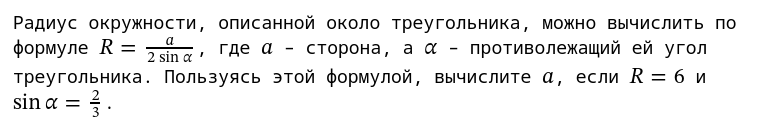
\includegraphics[width=1\linewidth]{506300-4-2.png}
} б) \\
\end{minipage}
\caption{Задачи, соответствующие шаблону 506300:
\\
а) исходная; б) сгенерированные}
\label{ris:506300}
\end{figure}



%%7 делится на две главы. Задача с чертежом коорд.оси (предвор сведения, разработанные библ функции, шаблоны)
\section{Задачи №7 ОГЭ (координатная прямая)}

\subsection{разработка функции}
Наиболее значимая часть работы — это разработка функций для визуализации координатной прямой и точек на ней. 
Была создана универсальная функция, позволяющая отображать засечки и подписи в разных режимах.

Одним из ключевых элементов реализации автоматической генерации заданий стала функция $coordAxis_drawMarkPoint$. Она предназначена для отрисовки различных типов меток на координатной оси и их подписей.

\subsection{Назначение функции}
Функция решает задачу визуализации точек и вспомогательных обозначений на оси,
что является неотъемлемой частью заданий ОГЭ и ЕГЭ по математике.
С помощью данной функции возможно изображать:
\begin{itemize}
    \item закрашенные точки (``dot''),
    \item выколотые точки (``emptyDot''),
    \item засечки (``line''),
    \item отсутствие метки (``nothing'').
\end{itemize}

\lstinputlisting[]{code/7/drawMarkPoint.js} 

\subsection{Интерфейс функции}
Функция имеет следующий набор параметров:
\begin{itemize}
    \item \texttt{ct}~--- графический контекст Canvas,
    \item \texttt{coord}~--- координата по оси X,
    \item \texttt{text}~--- подпись для метки,
    \item \texttt{markForm}~--- форма метки: \texttt{dot}, \texttt{emptyDot}, \texttt{line}, \texttt{nothing},
    \item \texttt{textPosition}~--- расположение подписи: под осью (\texttt{underAxis}), над осью (\texttt{overAxis}), на оси (\texttt{onAxis}),
    \item \texttt{options}~--- дополнительные параметры (шрифт, цвет текста, толщина линии, смещение).
\end{itemize}

\subsection{Алгоритм работы}
\begin{enumerate}
    \item Сохраняются текущие параметры отрисовки (\texttt{fillStyle}, \texttt{strokeStyle}, \texttt{font}, \texttt{lineWidth}).
    \item Устанавливаются новые параметры, переданные в \texttt{options}.
    \item В зависимости от параметра \texttt{markForm} рисуется выбранный элемент:
    \begin{itemize}
        \item точка~--- закрашенный круг,
        \item выколотая точка~--- окружность с заливкой белым цветом внутри,
        \item засечка~--- вертикальная черта,
        \item отсутствие~--- элемент не отрисовывается.
    \end{itemize}
    \item В зависимости от параметра \texttt{textPosition} подпись размещается под осью, над осью или на линии оси.
    \item Восстанавливаются исходные параметры графического контекста.
\end{enumerate}

 \texttt{coordAxis\_prepare}, что позволяет подготовить область для оси и рисует стрелку. И
\texttt{coordAxis\_drawAuto} она автоматически вычисляет масштаб оси и вызывает $coordAxis_drawMarkPoint$ для всех точек.


Функция \texttt{coordAxis\_prepare} выполняет подготовку холста для отрисовки горизонтальной координатной оси со стрелкой.
Она:
\begin{itemize}
  \item задаёт габариты рабочей области оси (\verb|width|, \verb|height|) и сохраняет их в контексте для последующего использования;
  \item вертикально центрирует ось (Ox) (смещение системы координат);
  \item настраивает стили (цвет линии и толщину) и рисует ось со стрелкой;
  \item бережно восстанавливает исходные графические параметры контекста.
\end{itemize}
Компонент рассчитан на дальнейшее использование вместе с $coordAxis_drawMarkPoint$ и $coordAxis_drawAuto$.

\lstinputlisting[]{code/7/prepare.js} 

\begin{description}
  \item[\texttt{ct}] графический контекст \verb|CanvasRenderingContext2D|.
  \item[\texttt{width}] ширина области оси в пикселях, по умолчанию (400).
  \item[\texttt{height}] высота области в пикселях, по умолчанию (100).
  \item[\texttt{strokeStyle}] цвет линии оси (интеграция со стилем проекта через \verb|om.primaryBrandColors[0]|).
  \item[\texttt{lineWidth}] толщина линии оси, по умолчанию (2).
\end{description}

Функция явно сохраняет текущие значения \verb|strokeStyle| и \verb|lineWidth| в локальные переменные
\verb|prevStroke| и \verb|prevLineWidth| и восстанавливает их к концу выполнения.  
Параметры \verb|ct.__coordAxisW| и \verb|ct.__coordAxisH| записываются в контекст как служебные метаданные — это упрощает доступ к габаритам при последующих рисованиях (например, при авторазметке меток).

Важно, что вызывается \verb|ct.translate(0, height/2)|: система координат сдвигается на половину высоты вниз, чтобы ось (Ox) оказалась по центру холста. Этот сдвиг является \emph{накопительным}; поэтому рекомендуется либо:
\begin{itemize}
  \item вызывать \verb|coordAxis_prepare| один раз в рамках одного цикла отрисовки, либо
  \item оборачивать работу в \verb|ct.save() ... ct.restore()|, если требуется многократная подготовка в одном контексте.
\end{itemize}

\verb|coordAxis_prepare| задаёт «сцену» — габариты, позицию оси и её визуальные атрибуты. Поверх этой сцены функции \verb|coordAxis_drawMarkPoint| и \verb|coordAxis_drawAuto| размещают метки и подписи.
 Такое разделение обязанностей упрощает поддержку кода: изменения оформления оси не затрагивают логику генерации и размещения меток.
Данная функция является частью связки:
    
Из особенностей можно подчеркнуть что функция поддерживает как закрашенные, так и выколотые точки, что позволяет формировать задания с открытыми и закрытыми интервалами.
Так же она восстанавливает исходные параметры, гарантирует корректную работу при множественной отрисовке. А так же есть возможность смещения текста по оси X , что помогает избежать наложений подписей.
\lstinputlisting[]{code/7/drawAuto.js} 


\subsection{Пример использования}
\begin{verbatim}
// Отрисовка закрашенной точки A с подписью под осью
coordAxis_drawMarkPoint(ct, 100, "A", "dot", "underAxis");

// Отрисовка выколотой точки B с подписью над осью
coordAxis_drawMarkPoint(ct, 200, "B", "emptyDot", "overAxis");
\end{verbatim}

Пример работы:
\lstinputlisting[]{code/7/314802.js} 
До:
После:
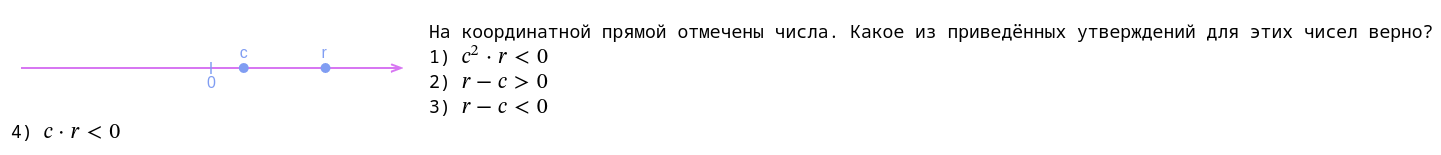
\includegraphics[width=0.4\textwidth]{314802-7-3.png}
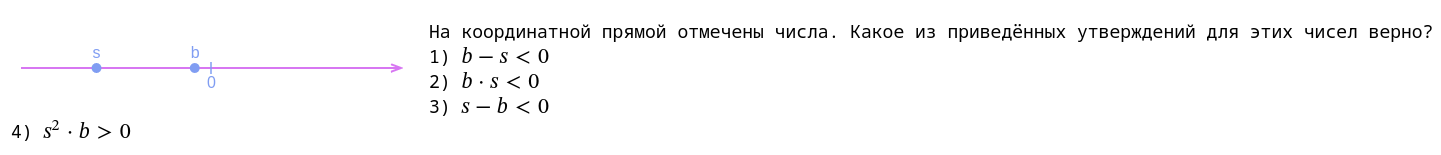
\includegraphics[width=0.4\textwidth]{314802-7-2.png}
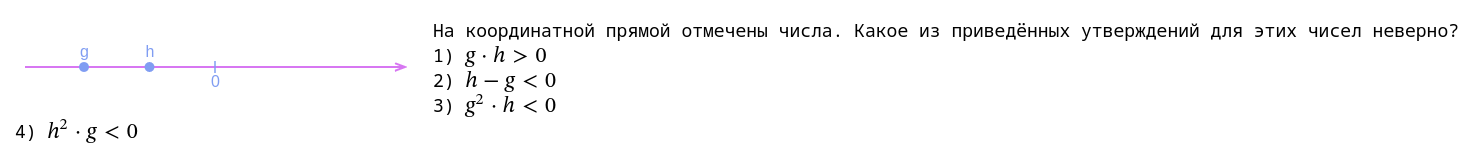
\includegraphics[width=0.4\textwidth]{314802-7-1.png}

\lstinputlisting[]{code/7/337301.js} 
До:
После:
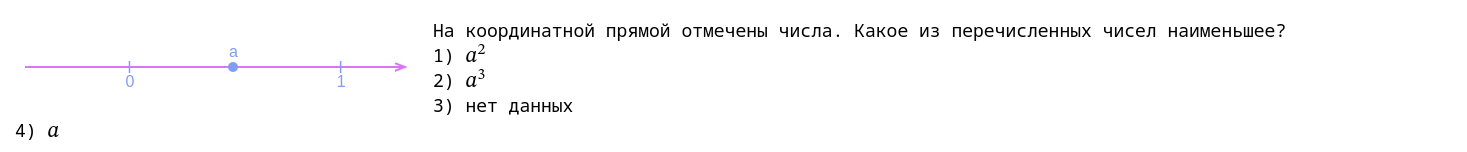
\includegraphics[width=0.4\textwidth]{337301-7-1.png}
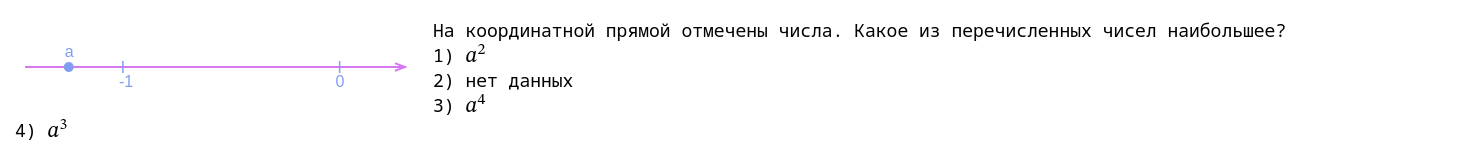
\includegraphics[width=0.4\textwidth]{337301-7-2.png}

%7 делится на две главы. Задача с чертежом коорд.оси (предвор сведения, разработанные библ функции, шаблоны)
% вторая - задача на сравнение чисел (как устроено округление,autoLateX )
\section{Задачи №7 ОГЭ (сравнение чисел)}
В проекте присутствует отдельный шаблон, посвящённый задачам на сравнение действительных чисел. 
Основная цель подобных заданий --- научить учащегося ориентироваться в числовой прямой, дробях и приближённых значениях корней.  

Так как в задачах встречаются как обыкновенные дроби, так и десятичные приближения квадратных корней, 
важно уметь корректно округлять результаты. Для этого используется метод \verb|toFixed(1)|, позволяющий оставить одно десятичное число. Например:

\begin{lstlisting}[language=JavaScript]
let correctVal = ((frac1 + frac2) / 2);
let correct = correctVal.toFixed(1).ts();
\end{lstlisting}
Здесь мы берём среднее значение между двумя дробями, а затем округляем его до одного знака после запятой, 
чтобы получить корректный ответ, который предлагается ученику.  
Пример:
\lstinputlisting[]{code/7/205843.js} 
До:
После:
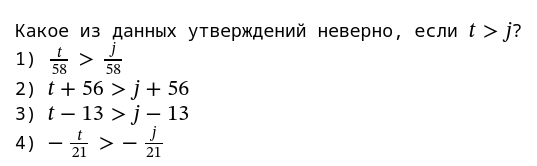
\includegraphics[width=1\textwidth]{205843-7-3.png}
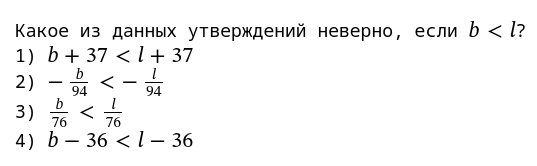
\includegraphics[width=1\textwidth]{205843-7-2.png}
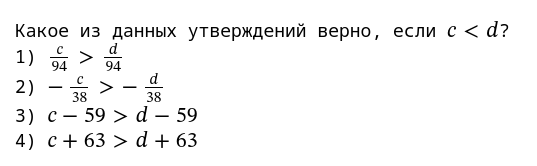
\includegraphics[width=1\textwidth]{205843-7-1.png}

Для проверки знаний учащегося необходимо не только предъявить правильный ответ, 
но и сформировать несколько правдоподобных «ловушек». 
В нашем проекте это реализовано через генерацию трёх ложных ответов. 
Ложные варианты создаются с помощью небольших шумов (\verb|noise|), добавляемых к правильному значению.  

\begin{lstlisting}[language=JavaScript]
let wrong = new Set();
while (wrong.size < 3) {
    let noise = slKrome([0], -7, 7) * 0.1;
    let candidate = +(correctVal + noise).toFixed(1);

    if (candidate <= 0 || candidate > frac1 && candidate < frac2 
        || candidate === +correctVal.toFixed(1)) {
        continue;
    };
    wrong.add(candidate.ts());
}
\end{lstlisting}

Таким образом, в итоговом задании всегда предлагается \textbf{4 варианта ответа}: один правильный и три ложных.  

После задания параметров задачи и вариантов ответа вызывается функция \verb|AtoB(3)|. 
Она отвечает за автоматическую генерацию списка вариантов с правильным ответом, расположенным случайным образом.  

\begin{lstlisting}[language=JavaScript]
NAtask.setTask({
    text: 'Какое из следующих чисел заключено между числами ${' + text1 + '}$ и ${' + text2 + '}$?',
    answers: correct,
    wrongAnswers: Array.from(wrong)
});

AtoB(3, { autoLaTeX: true });
\end{lstlisting}

Чтобы не окружать каждую формулу знаками \verb|$...$|, используется параметр \verb|{ autoLaTeX: true }|. 
Это позволяет сразу включать математические выражения (например, дроби и корни) прямо в текст задачи. 
В результате формулы корректно отображаются в интерфейсе без дополнительной ручной разметки.  

В результате ученик видит задачу: 
\textit{«Какое из следующих чисел заключено между числами …?»}, 
к которой автоматически предлагаются четыре варианта ответа.  
% расфосовать задачи чуть более аккуратно и с фотографиями до /после
Пример:

\lstinputlisting[]{code/7/311420.js} 
До:
После:
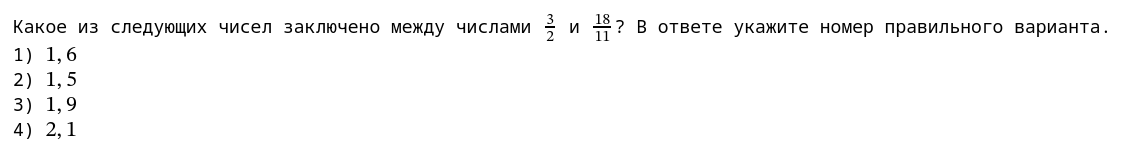
\includegraphics[width=1\textwidth]{311420-7-1.png}
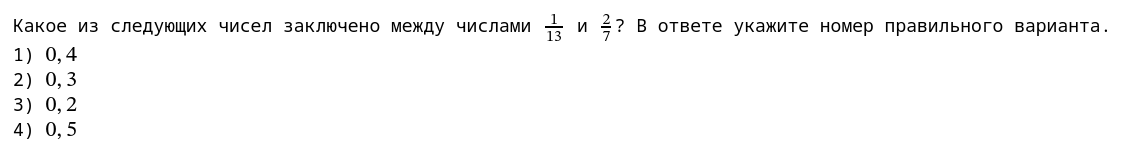
\includegraphics[width=1\textwidth]{311420-7-2.png}

\lstinputlisting[]{code/7/317132.js} 
До:
После:
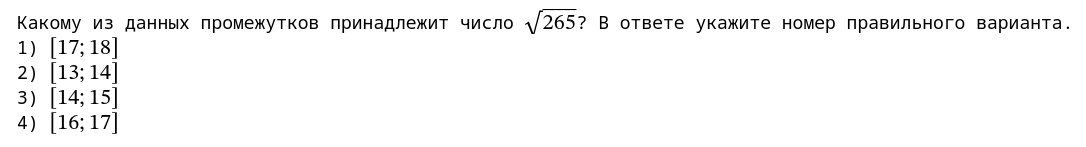
\includegraphics[width=1\textwidth]{317132-7-1.png}
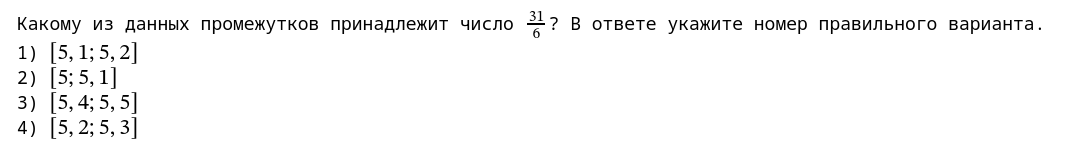
\includegraphics[width=1\textwidth]{317132-7-2.png}

Исходная задача:
Сгенрированная задача:


%\begin{figure}[h]
%\center{\includegraphics[width=1\linewidth]{image}}
%\caption{Зависимость сигнала от шума для данных.}
%\label{ris:image}
%\end{figure}


На рис.~\ref{ris:317132} представлены исходная и сгенерированные задачи по шаблону №317132.


\begin{figure}[h]
\begin{minipage}[h]{0.95\linewidth}
\center{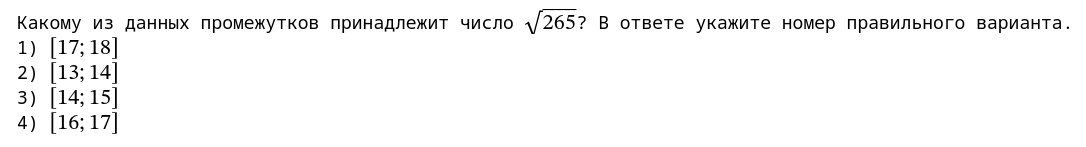
\includegraphics[width=1\linewidth]{317132-7-1.png}} \\а)
\end{minipage}
\vfill
\begin{minipage}[h]{0.95\linewidth}
\center{%
    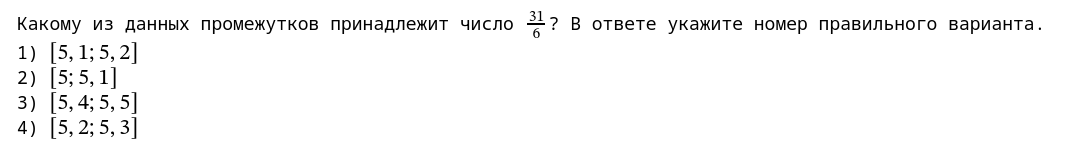
\includegraphics[width=1\linewidth]{317132-7-2.png}
    \\
    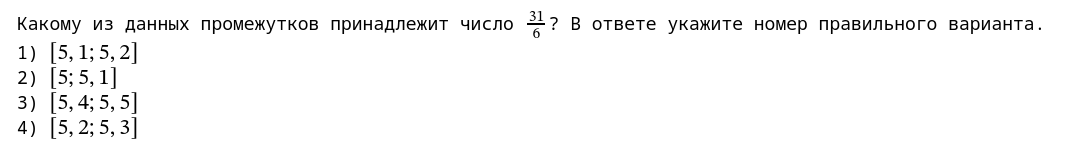
\includegraphics[width=1\linewidth]{317132-7-2.png}
} б) \\
\end{minipage}
\caption{Задачи, соответствующие шаблону 317132:
\\
а) исходная; б) сгенерированные}
\label{ris:317132}
\end{figure}


%%%%%%
%%%%%%

Ура?

\section*{Заключение}
\addcontentsline{toc}{section}{Заключение}
В ходе выполнеия курсовой работы за 3 курс был покрыт открытый банк заданий ФИПИ по темам:
		      \begin{itemize}
			      \item Текстовые задачи (на смекалку) — 12 шаблонов принято.
			      \item Текстовые задачи (проценты и дроби) — 29 шаблонов принято.
			      \item Преобразования выражений — 29 шаблонов (25 принято 4 на внутреннем рецензировании).
			      \item Задачи с прямыми — 10 шаблонов принято. (3 с рисунком и 7 на сравнение чисел )
		      \end{itemize}

В ядро проекта добавлены: 
\begin{itemize}
    \item Функции, упрощающие написание шаблонов по теме «Координатная прямая».
    \item r2 % как это описать, как это описать....
\end{itemize}

А также сокращён технический долг проекта.

Все добавленные в проект задания можно использовать для составления контрольных работ, проведения текущего контроля знаний учащихся, подготовки к ЕГЭ.~\cite{chas-ege}

В будущем планируется добавить% в проект класс плоских геометрических фигур и использовать в заданиях по теме «Планиметрия» динамические изображения.




\begin{thebibliography}{6}
	\bibitem{chas-ege} Тренажёр "Час ЕГЭ". – URL: https://math.vsu.ru/chas-ege/sh/katalog.html
	\bibitem{fipi}Федеральный институт педагогических измерений. – URL:  https://fipi.ru/ege/otkrytyy-bank-zadaniy-ege
	\bibitem{egemath}Открытый банк задач ОГЭ по математике. – URL:  https://oge.sdamgia.ru/?Redir=1
	\bibitem{egemath}Открытый банк задач ЕГЭ по математике. Базовый уровень. – URL:  https://mathb-ege.sdamgia.ru
	\bibitem{ege} Единый государственный экзамен. – URL:  https://ru.wikipedia.org/wiki/Единый\_государственный\_экзамен
	\bibitem{sdamgia}Решу ЕГЭ - Сдам ГИА. – URL: https://ege.sdamgia.ru/problem?id=27074
\end{thebibliography}

\include{applications.tex}

\end{document}

